

% Lösungen ein- bzw. ausblenden
\newif\ifloesung
\loesungtrue

% Sprache wechseln
\newif\ifenglisch
\englischtrue
%\englischfalse

\documentclass[a4paper,12pt,ngerman]{article}
\usepackage[utf8]{inputenc}
\usepackage[T1]{fontenc}     % Um die Zeichen korrekt zu kodieren
\usepackage[ngerman]{babel}
\usepackage{amssymb}  % für \Box
\usepackage{fancyhdr}
\usepackage{setspace}
\usepackage{framed}
%\usepackage{xcolor}
\usepackage{hhline}
\usepackage{longtable}
\usepackage{array}     % für m{} etc. in Tabellen
%\usepackage{booktabs}  % für \addlinespace[2ex] in Tabellen
\usepackage{graphicx}
\usepackage[export]{adjustbox}
\usepackage{caption}
\usepackage{subcaption}
%\usepackage{hyperref}  % für \autoref{...}
\usepackage{lastpage}  % für thelastepage im Header
\usepackage{paralist}  % compactenum in Unteraufgaben
\usepackage{enumitem}  % Anpassbare Enumerates/Itemizes
%\usepackage{pstricks}  % Tex-Graphiken exportiert von Dia
\usepackage{tikz}    
\usepackage{xparse}    % für neue Befehle mit variabler Anzahl von Parametern (hier \lsg)
\usepackage{soul}      % zum "verstecken" von Lösungstext
%\usepackage[plainpages=false, pdfpagelabels,colorlinks=true, pdfstartview=FitV, linkcolor=blue, citecolor=blue, urlcolor=blue]{hyperref}
\usepackage{listings}
\usepackage{eurosym}   % für das Euro-Symbol
\usepackage{verbatim}
%\usetikzlibrary{positioning,shapes,shadows,arrows.meta,calc}
\usepackage{lipsum}
\usepackage[most]{tcolorbox}

% % % % % % % % % % % % % % % % % % % % % % % % % % % % %
% Befehle zum Ein- und Ausblenden von Lösungen
%

\ifloesung
	\NewDocumentCommand\lsg{+m +g}{%
		\textcolor{red}{#1}
	}
	\newcommand{\nlsg}[1]{}
\else
	\NewDocumentCommand\lsg{+m +g}{%
		\IfNoValueF{#2}
			{#2}
			{}
	}
	\newcommand{\nlsg}[1]{#1}
\fi

% Jedes Zeichen innerhalb von \geheim{...} entfernen
% wenn die Zeichen durch etwas anderes (z.B. ?) ersetzt
% werden sollen dann \phantom{\the\SOUL@token} ersetzen 
% (z.B. durch ?)
% benötigt \usepackage{soul}
\makeatletter
\DeclareRobustCommand{\geheim}{%
  \SOUL@setup
  \def\SOUL@everytoken{%
    \phantom{\the\SOUL@token}}\SOUL@}
\makeatother

% % % % % % % % % % % % % % % % % % % % % % % % % % % % %

% % % % % % % % % % % % % % % % % % % % % % % % % % % % %
% Konfiguration der Codeausgabe mit listings
%
%\usepackage{pxfonts}  % erlaube \ttfamily in bold, geht derzeit nicht in meinem MikTex unter Windows  
\renewcommand{\ttdefault}{pcr} % Courier font auswählen, der bold erlaubt, (Alternative zu pxfonts)
\lstset{basicstyle=\ttfamily}
%\lstset{keywordstyle=\bfseries} % ist Default
% \bf hinzufügen, wenn es bold sein soll
% gilt auch für Code im Text
\lstset{keywordstyle=\bfseries}
%\lstset{keywordstyle=\bfseries\ttfamily\underbar}
%\lstset{keywordstyle=\color{blue}\ttfamily}
\lstset{stringstyle=\it}
%\lstset{stringstyle=\color{red}\ttfamily}
%\lstset{commentstyle=\ttfamily\itstyle}
%\lstset{commentstyle=\color{green}\ttfamily}
\lstset{tabsize=4}
\lstset{showtabs=false}
\lstset{language=C++}
\lstset{morekeywords={ostringstream, istringstream, stringstream, ostream}}
%\lstset{showspaces=false, 
%        showtabs=false, tab= , 
%		 keywordstyle=\blue\bfseries, 
%		 commentstyle=\it\color{greenf},%
%        showstringspaces=false, framexleftmargin=5mm, 
%		 frame=none, numbers=none, numberstyle=\tiny, 
%		 stepnumber=1, numbersep=5pt,%
%        texcl=true,escapechar=!
%}
% automatischen Zeilenumbruch erlauben  \lstset{breaklines=true}  
% automatischer Zeilenumbruch nur bei Whitespace              
\lstset{breakatwhitespace=false}
\lstset{showstringspaces=false,
        commentstyle=\color{black} 
%        morecomment=[l]{//}
}
% Coder der Lösung in rot oder ausgeblendet
\ifloesung
\lstset{morecomment=[l][\color{red}]{//=},
		morecomment=[s][\color{red}]{//+}{//-},
		morecomment=[s][\color{red}]{//l\{}{//l\}},		
		morecomment=[s][\color{red}]{/*l\{*/}{/*l\}*/}
}
\else
% mit [is] wird der Kommentar ignoriert und nicht ausgegeben ==> Platz für Lösung einplanen
% [il] funktioniert nicht, löscht alles Folgende
\lstset{morecomment=[is]{//=}{.},
	 	morecomment=[is]{//+}{//-},
		morecomment=[is]{//l\{}{//l\}},	 	
	 	morecomment=[is]{/*l\{*/}{/*l\}*/}
}
\fi
% Umlaute in Listings zu erlauben
\lstset{literate=      
{Ö}{{\"O}}1       
{Ä}{{\"A}}1
{Ü}{{\"U}}1
{ß}{{\ss}}2
{ü}{{\"u}}1
{ä}{{\"a}}1
{ö}{{\"o}}1
{~}{$\sim$}{1}     % hochgestellte Tilde in eine in Mitte
                   % gestellte Tilde umwandeln
}
% Programmcode im Text
\newcommand\pct[1]{\lstinline!#1!}

% % % % % % % % % % % % % % % % % % % % % % % % % % % %

% % % % % % % % % % % % % % % % % % % % % % % % % % % %
% Konfiguration für tikz
%

%\definecolorset{rgb}{}{}%
%{lightyellow,1,1,0.6;%
% lightblue,0.529,0.81,1;%
% lightred,1,0.6,0.6;%
% greenf,0,0.5647,0%
%}

%\pgfrealjobname{pruefung}
%\usetikzlibrary{shapes,arrows,intersections,backgrounds}
%\usetikzlibrary{decorations.markings, decorations.pathmorphing,patterns,snakes}
%\usetikzlibrary{circuits.ee.IEC, circuits.logic.IEC}
%tikzstyle{ST2style} = [auto, line width=1pt, >=stealth]

%\tikzstyle{input}    = [coordinate]
%\tikzstyle{output}   = [coordinate]

%\tikzstyle{blockS}   = [fill=lightyellow, draw=black, rectangle, minimum height=4ex, minimum width=3em] % Block Strecke ; normal hoch
%\tikzstyle{blockBS}  = [style = blockS,  minimum height=6ex] % Block Strecke ; höher für Bruch
%\tikzstyle{blockR}   = [style = blockS,  fill=cyan!20]       % Block Regler ; normal hoch
%\tikzstyle{blockBR}  = [style = blockR, minimum height=6ex] % Block Regler ; höher für Bruch

%\tikzstyle{sumS}     = [draw=black, fill=lightyellow, circle, inner sep=0pt,minimum size=3mm]  % Summationsstelle Strecke
%\tikzstyle{sumR}     = [style = sumS, fill=cyan!20]  % Summationsstelle Regler

%\tikzstyle{connectiondot} = [draw=black, fill=black, circle, inner sep=0pt,minimum size=1mm]  % Punkt zum Verbinden von Signallinien
%\tikzstyle{connectiondotvector} = [style = connectiondot, minimum size=2mm]  % Punkt zum Verbinden von Signallinien

%\tikzstyle{vectorline} = [line width=1pt, double]
%\tikzstyle{pinstyle} = [pin edge={to-,ST2style, black}]

% % % % % % % % % % % % % % % % % % % % % % % % % % % % %

\renewcommand{\bf}{\bfseries}

\newcommand{\anzblaetter}{\pageref{LastPage}}

% % % % % % % % % % % % % % % % % % % % % % % % % % % % %
% Definition des Aufgabenlayouts und -nummerierung
%

% Der Zähler aufgabe als Unterzähler von chapter
% zählt die Aufgaben in einem Kapitel
% Mit \aufgabe{Titel} wird eine neue Aufgabe begonnen.
\newcounter{aufgabe}
\setcounter{aufgabe}{0}
\renewcommand{\theaufgabe}{\arabic{aufgabe}}
\newenvironment{aufgabe}[2]%
	{\refstepcounter{aufgabe}
    \vskip 6pt plus 3pt minus 3pt
    \ifenglisch
      {\bf\large Question \arabic{aufgabe}: #1 \hfill (#2 Min.)}
    \else
      {\bf\large Aufgabe \arabic{aufgabe}: #1 \hfill (#2 Min.)}
    \fi
   	%\\
   	%\vskip 3pt plus 3pt minus 3pt	
	}%
	{}
% Umgebung für Liste der Unteraufgaben
\newlist{aufgabenliste}{enumerate}{3}
\setlist[aufgabenliste]{topsep=0pt,partopsep=0pt,itemsep=0pt,parsep=4pt}
\setlist[aufgabenliste,1]{label=\theaufgabe.\arabic*}
\setlist[aufgabenliste,2]{label=\alph*}
\setlist[aufgabenliste,3]{label=\roman*}
\newenvironment{unteraufgaben}%
    { \begin{aufgabenliste} }%
    { \end{aufgabenliste} }

% % % % % % % % % % % % % % % % % % % % % % % % % % % % %

% % % % % % % % % % % % % % % % % % % % % % % % % % % % %

% Text für englische Sprache für bilinguale Klausuren hervorheben
\newcommand{\engl}[1]{\emph{#1}}

% Ein paar Variablen im Logfile ausgeben
\newcommand{\vars}{%
\message{****hoffset = \the\hoffset}
\message{****voffset = \the\voffset}
\message{****headheight = \the\headheight}
}

%\newdimen\remainingheight
%\newcommand*{\calcremainingheight}{%
%    \remainingheight\dimexpr\pagegoal-\pagetotal-\baselineskip-\parskip
%}

\newdimen\remainingheight
\newcommand*{\calcremainingheight}{%
    \ifdim\pagegoal=\maxdimen
        \remainingheight\dimexpr\textheight-0.4pt\relax
    \else
        % edit 2: replaced -\baselineskip by -\lineskip-0.4pt
        % edit 3: removed -\parskip
        \remainingheight\dimexpr\pagegoal-\pagetotal-\lineskip-0.4pt-\parskip\relax
    \fi
}



%
% page layout
%
% Äußerer Seitenrand = one inch + \hoffset 
\hoffset = 0pt
% Oberer Seitenrand = one inch + \voffset
\voffset = -1cm
% Abstand zwischen äußerem Seitenrand und Text
% auf ungeraden Seiten
\oddsidemargin = 0pt
% Abstand zwischen äußerem Seitenrand und Text
% auf ungeraden Seiten
\oddsidemargin = 0pt
% Abstand zwischen oberem Seitenrand und Header
\topmargin = 0pt
% Höhe des Headers der ersten Seite
\headheight = 151pt
% Abstand zwischen Header und Text
\headsep = 0pt
% Texthöhe
\textheight = 205mm
% Textbreite
\textwidth = 170mm
% Abstand vom Text zu den Marginalien
% \marginparsep = 11pt 10 
% Breite der Marginalien
% \marginparwidth = 54pt
% Abstand Text zu Unterkante Footer
\footskip = 2pt 
% Papierbreite
%\paperwidth = 597pt 
% papierhöhe
%\paperheight = 845pt

% Einzug von Absätzen
\parindent 0mm
% Abstand von Absätzen
\parskip .6\baselineskip plus 1pt
%
% commands
%
\renewcommand{\bottomfraction}{1}
\renewcommand{\topfraction}{1}
\renewcommand{\textfraction}{0}
\textfloatsep1ex plus 1ex minus.5ex
%
% avoid date
%
%\date{}
%
% to get more tolerance (mir)
%
\tolerance800
\emergencystretch2em
\doublehyphendemerits5000
\hfuzz0pt
\leftskip0pt minus 1pt
\rightskip0pt minus 1pt

%\setlength\parskip{.4\baselineskip plus5pt minus2pt}

%
%  neuer pagestyle
%
% % % % % % % % % % % % % % % % % % % % % % % % % % %
%
% Header

% gemeinsame Infos:
\newcommand{\halbjahr}{{\bf Summer Term 2016}}
\newcommand{\studiengangi}{Automotive Systems}
\newcommand{\studiengangii}{}
\newcommand{\studiengangiii}{}
\newcommand{\semesteri}{ASM-SB}
\newcommand{\semesterii}{}
\newcommand{\semesteriii}{}
\newcommand{\fach}{ Reliable Embedded Systems }
\newcommand{\lecture}{{\bf Distributed Real-Time Systems }}
\newcommand{\fachnummer}{}
\newcommand{\hilfsmittel}{closed book apart from \par 2 sheets of DIN-A4 paper}
\newcommand{\dozent}{Agrawal}
\newcommand{\dauer}{60 minutes}

\newlength{\headerspaltenbreite}
\setlength{\headerspaltenbreite}{8.5cm}

% Header für die erste Seite
\newcommand{\firstpageheader}{
{\bfseries University of Applied Sciences Esslingen \hfill\hfill Faculty Graduate School}\\
\begin{small}
{ % Änderung lokal halten
% Platz zwischen \hline und Text einfügen
\setlength{\extrarowheight}{1.5pt}
\begin{tabular}{|lm{\headerspaltenbreite}|ll|}\hline
\multicolumn{2}{|l|}{\halbjahr} & Page No.:  & \thepage\ of \anzblaetter \\\hline
Programme:   & \studiengangi  & Semester:   & \semesteri   \\\hline
%               & \studiengangii &             & \semesterii  \\
%               & \studiengangiii&             & \semesteriii \\\hline
Module:  & \fach          &             & \\
Lecture: & \lecture       & Lecturer:     & \dozent      \\\hline
Mode:   & \hilfsmittel   & Duration:      & \dauer       \\\hline
Name:          &                & Student ID: &          \\[3ex]\hline               
\end{tabular}
}
\end{small}
}
% Header für erste Seite setzen
\fancypagestyle{firstpagestyle}{
   \fancyhf{}
   \chead{\firstpageheader}
   \cfoot{} %\cfoot{\thepage}
}
%\thispagestyle{firstpagestyle}

% Header für die folgenden Seiten
\newcommand{\nextpageheader}{
\begin{small}
{ % Änderung lokal halten
% Platz zwischen \hline und Text einfügen
\setlength{\extrarowheight}{1.5pt}
\begin{tabular}{|lm{9.6cm}|ll|}\hline
\multicolumn{2}{|l|}{\halbjahr} & Page No.:  & \thepage\ of \anzblaetter \\\hline
Lecture:  & \lecture          & Semester: & \semesteri  \\\hline
%Name:          &                & Student number: & \\[3ex]\hline               
\end{tabular}
}
\linebreak
\linebreak
\end{small}
}

\pagestyle{fancy}
% Header leeren
\fancyhf{}
\chead{\nextpageheader}
\cfoot{} %\cfoot{\thepage}
%\cfoot{\small\it Bitte geben Sie alle Aufgabenblätter wieder ab!}
% kein weiterer horizontaler Strich
\renewcommand{\headrulewidth}{0pt}
\renewcommand{\plainheadrulewidth}{0pt}
\newcommand{\degree}{\ensuremath{^\circ}}



% \lsg{#1} zeigt #1 an, wenn \loesungtrue
% \lsg{#1}{#2} zeigt #1 an, wenn \loesungtrue und #2 andernfalls, dabei dürfen #1 und #2 nicht zu kompliziert sein
% \nlsg{#1} gibt #1 an, wenn \loesungfalse

% In Source Code mit listings wird für Code
% von //+  bis //- und /*+*/ bis /*-*/ sowie
% von //l{  bis //l} und /*l{*/ bis /*l}*/ 
% sowie in der Zeile nach //= mit abschließendem .
% die Textanzeige unterdrückt, wenn \loesungfalse

% Pfad, wo die CPP- u. HPP-Dateien zu finden sind
\newcommand{\Code}{Code}

\begin{document}

% Auf der ersten Seite den vollständigen Header nutzen
\thispagestyle{firstpagestyle}


%
\aufgabe{}{1}

An RT entity changes its value periodically according to 
\begin{displaymath} 
y(t) = A_{0}.\sin(2\pi ft) 
\end{displaymath} 
with amplitude $A_{0}$ and frequency f . What is the maximum permissible frequency $f_{max}$ for the entity value if the entity is sampled with a period of $T_{sample}$ = 1 msec, and the maximum change of value
between two sampling points should never exceed 0.1\% of the full range value?

\begin{tikzpicture}
\node (rect) at (0,0) [draw, text width=17 cm, minimum height=12cm]{};
\node[below right, text width=17 cm] at (rect.north west) {
    \lsg{
    Please sketch a model here
    }
   };
\end{tikzpicture}

\aufgabe{}{1}

Explain the difference between safety and reliability in hard real-time systems.

\aufgabe{}{2}

Explain the term “signal conditioning” in hard real-time systems.

\aufgabe{}{2}

Discuss the advantages and disadvantes of a distributed architecture vs. a centralized
architecture in terms of cost, reliability, and safety.


\aufgabe{}{2}

Explain the terms offset, drift, drift rate, precision, and accuracy in the context of real-time
clocks. Use a sketch if appropriate.

\aufgabe{}{4}

 Assume k clocks behave maliciously faulty. How many clocks N do you need at least to
achieve clock synchronisation?

\pagebreak
\headheight = 78pt

\aufgabe{}{10}

Explain the difference between the accuracy and precision of a clock.

\aufgabe{}{3}

 Explain the difference between state correction and rate correction for distributed clocks

\aufgabe{}{5}

Describe the structure of a node. Why is it important to distinguish between the i-state and
the h-state of a node in an embedded system?

\aufgabe{}{5}

 What is the difference between a parametric RT image and a phase-sensitive RT image?
How can we create parametric RT images?

\pagebreak


\aufgabe{}{5}

Calculate the action delay in a distributed system with the following parameters:
dmax=10msec, dmin=2msec,
and a) no global time available, granularity of local time is 20$\mu$sec
and b) global time with granularity of 30$\mu$ sec.

\aufgabe{}{5}

What are the problems with event observations?

\pagebreak

\aufgabe{}{5}

What are the basic techniques for error detection?

\aufgabe{}{5}

Given a bandwidth of 10 Mbit/sec, a channel length of 1000 m, and a message length of 100
bits, what is the limit of the protocol efficiency that can be achieved at the media access
level of a bus system?

\aufgabe{}{5}

Given are four tasks which access resources (A,B,C):
$\tau$ 1 (r 0 = 10, C = 4, Prio=4; [A;1]), where the task executes for two time units, and then requests
the resource A.
$\tau$ 2 (r 0 = 7, C = 4, Prio=3; [A;1][B;1]), where the task executes for one time unit, and then
requests the resource A, and thereafter B.
$\tau$ 3 (r 0 = 4, C = 4, Prio=2; [B;1][C;1]), where the task executes for one time unit, and then
requests the resource B, and thereafter C.
$\tau$ 4 (r 0 = 4, C = 4, Prio=1; [A;5[B;2]][C;1]), where the task executes for two time units, then
requests the resource A, holds it for one time unit, and then makes a nested request for resource
B, and then requests C.
Notation: r 0 is the release or request time, C is the execution time, Prio is the priority of the tasks
(higher number means higher priority). [A;5] means request to resource A for five time units.
[A;a[B;b]] means a nested critical sections, where the usage of A includes in turn the usage of B,
and time a includes time b.
This task set shall be scheduled with two different resource access protocols.
3.1 Construct the schedule for this task set using the priority inheritance protocol. Use the the
diagram furnished below. On the first four lines draw the schedule of each task as if there
were no other tasks. On the last line, draw the resulting schedule. Do not use a different
diagram template.

3.2  Construct the schedule for this task set using the priority ceiling protocol. On the first
four lines draw the schedule of each task as if there were no other tasks. On the last
line, draw the resulting schedule. Use the diagram provided below. Do not use your own
diagram templates


3.3 Take a look at another periodic task set with periods Ti and the following parameters:
Is it possible to create a schedule that meets all deadlines using the rate monotonic
algorithm (RMA)? Please explain.
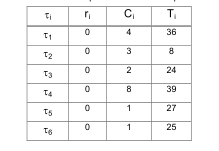
\includegraphics[width=0.7\textwidth]{master-exam-2009/2009_RMA}


3.4  Construct the schedule (mark using X) for the task set above and priority driven RMA into
the table below (two lines, second table is continuation of first table):

3.5 For the task set given in 3.3 consider the context switch time (the time it takes to
switch from execution of one task to another). This time shall take 0.8 time units, including
the start of the first job. Is it possible to create a valid schedule under these conditions?
Please explain.




%\aufgabe{}{1}

 Give an example for an end-to-end protocol in the context of a distributed real-time system.
Why would you have to use an end-to-end protocol at the interface between a computer
system and the controlled object?

\aufgabe{}{1}

State three functional requirements for real-time systems.

\aufgabe{}{2}

An average car is operated about 400 hours per year. Compute the permissible MTTF if one
out of one thousand cars may fail to provide the requested service throughout that year.
Would such a car be considered a system with an ultrahigh reliability requirement? Please
explain.

\aufgabe{}{2}

Why can there be conflicts between reliability and maintainability? Please explain.

\aufgabe{}{2}

Discuss the advantages and disadvantages of an event-triggered communication system vs.
a time triggered communication system. What would you prefer for ultra-dependable
systems, and why?

\aufgabe{}{4}

Explain the two failure modes of a clock.

\pagebreak
\headheight = 78pt

\aufgabe{}{10}

 How many binary digits (bits) would a digital counter need, if it was to directly measure a
time interval of 1 hour with a digitization error of less than 10 nsec?

\aufgabe{}{3}

Assume you need to measure a time interval with a precision of 10 nsec, where the start
event and the end event can origin from different nodes, and the node clocks are
synchronized to a global clock. What frequency must your node clocks at least have?


\aufgabe{}{5}

 Given a latency jitter of 10 $\mu$sec, a resynchronization period of 100 msec, and a clock drift
rate of $10^{-6}$ sec/sec, what precision can be achieved by the FTA algorithm in a system with
5 clocks where 1 clock could be malicious ($\mu$(5,1) = 1,5)?

\aufgabe{}{5}

Please explain why it is difficult to determine the WCET of processes in a hard-real time
system. State three methods that have been advised to determine WCET, and discuss their
limitations.

\pagebreak


\aufgabe{}{5}

 What is an observation in the context of real-time systems? Explain the two major types of
observations and discuss their advantages and disadvantages.

\aufgabe{}{5}

Calculate the action delay in a distributed system with the following parameters:
d$_{max}$=10msec, d$_{min}$=2msec,
and a) no global time available, granularity of local time is 50 $\mu$sec
and b) global time with granularity of 100 $\mu$sec.


\pagebreak

\aufgabe{}{5}

What kind of redundancy would you employ if you needed to detect errors caused by
independent software faults and by transient and permanent physical hardware faults?


\aufgabe{}{5}

What is triple modular redundancy (TMR)?

\aufgabe{}{5}

Fault tolerance can be implemented by two fail-silent nodes or by Triple Modular
Redundancy (TMR). Discuss the advantages and disadvantages of each approach.

\aufgabe{}{5}

Given a bandwidth of 1 MBits/sec, a channel length of 100 m and a message length of 64
bits, what is the limit of the protocol efficiency that can be achieved at the media access
level of a bus system?

\aufgabe{}{5}

Explain the role of the three time-outs in the ARINC 629 protocol. Is it possible for a collision
to occur on an ARINC 629 bus?

\aufgabe{}{5}

What mechanism helps to ensure the fail-silence of a TTP controller in the temporal
domain?

\aufgabe{}{5}

 Estimate the average and worst-case response time of a TTP/C system with 8 FTUs, each
one consisting of two nodes that exchange messages with 10 data bytes on a channel with a
bandwidth of 10 MBit/s. Assume that the interframe gap is 8 bits.

\aufgabe{}{5}

Explain the difference between polling and sampling.

%\aufgabe{}{1}

Sketch a simple model of a real-time system and partition it into three important parts. Name
each cluster and the interfaces between them.

\aufgabe{}{1}

What is the difference between a real-time image and a real-time entity?


\aufgabe{}{2}

Hard disk drives are often advertised with very high MTBFs. Some manufacturers have
switched to a different specification, the annual failure rate (AFR). The AFR is defined as
that percentage of a large number of disc drives that exhibit a defect when continuously
being run for a year.
What is the MTBF for a hard disc drive when the observations of the last year gave an AFR
of 0.73%, that is 0.73% of all disc drives that had been running continuously for a year
exhibited a defect?


\aufgabe{}{2}

Is real-time computing equivalent to fast computing? What is the main goal in the design of
real-time computing systems? Please discuss briefly.


\aufgabe{}{2}

 The start of an injection in a modern combustion engine must be controlled to better than $1\deg$,
to adhere to environmental standards. The idle motor speed of an engine is 800 rpm, the
maximum rate is 4500 rpm. The maximum change in motor speed in case of a load change
is 1500 rpm/sec.
a) Compute the maximum temporal accuracy for the start of the injection.
b) Compute for a one-cylinder four cycle engine at constant rpm the minimum time that is
available for the computation of the injection time. A four cycle engine needs to inject
only every other full crankshaft turn. Assume that there are no other processes running
on the computer calculating the injection time.
c) When the injection time is calculated early, it can become imprecise due to a change in
rpm during this time. Compute how far in advance the injection time can be calculated
without violating the $1\deg$ limit, assuming a maximum motor speed change. Assume for
your calculation that the computation doesn’t take any time at all.


\aufgabe{}{4}

Explain the three different types of orders with regard to alarms in a distributed real-time
system. Which of the orders implies another?


\pagebreak
\headheight = 78pt

\aufgabe{}{10}

How can a sparse time base help to avoid agreement protocols?


\aufgabe{}{3}

Assume you have node clocks running at a frequency of 100 MHz. What precision can you
achieve when measuring a time interval, where the start event and the end event can origin
from different nodes, and the node clocks are synchronized to a global clock?

\aufgabe{}{5}

Given a resynchronization period of 500 msec, and a clock drift rate of $10^{-6}$ sec/sec, what
latency jitter can be tolerated to achieve a precision of $20\mu$sec using the FTA algorithm in a
system with 5 clocks where 1 clock could be malicious ($\mu$(5,1) = 1,5)?


\aufgabe{}{5}

Please explain the difference between a simple task (S-task) and a complex task (C-task).
\pagebreak


\aufgabe{}{5}

 What is a history state? Please explain with an example.

\aufgabe{}{5}

Calculate the action delay in a distributed system with the following parameters:
dmax=20msec, dmin=5msec,
and a) no global time available, granularity of local time is 100 $\mu$sec
and b) global time with granularity of 500 $\mu$sec.

\pagebreak

\aufgabe{}{5}

When is a set of nodes replica determinate?


\aufgabe{}{5}

What is state estimation?

\aufgabe{}{5}

Explain the terms fault, error, an failure.

\aufgabe{}{5}

Given a bandwidth of 10 MBits/sec, a channel length of 200 m and a required protocol
efficiency of 90%, what is the maximum message length in bit that can be implemented by
the media access level of a bus system


\aufgabe{}{5}

What mechanism can lead to thrashing? How should you react in an event-triggered system
if thrashing is observed?


\aufgabe{}{5}

How can one distinguish between a Fireworks byte and a data byte in the TTP/A protocol?

\aufgabe{}{5}

 Calculate the data efficiency of a TTP/A system that consists of 5 nodes where each node
sends periodically a two byte message (user data). Assume that the intermessage gap
between the Fireworks byte and the first data byte is 4 bitcells, and the intermessage gap
between two successive data bytes is two bitcells. The gap between the end of one round
and the start of the next round is 6 bitcells.

\aufgabe{}{5}

Explain three major problems that we encounter in interrupt-driven software.


%\aufgabe{}{1}

One important parameter for many real-time computer programs is the WCET. Why is it
difficult to obtain the WCET? Give as many reasons as you can think of.

\aufgabe{}{1}

Explain the term “composability”. Give examples.

\aufgabe{}{2}

Explain the term “error containment region”.

\aufgabe{}{2}

What types of failures can a physical clock exhibit? Please explain briefly.

\aufgabe{}{2}

What are the basic techniques for error detection?

\aufgabe{}{4}

 What are the advantages of having a global time available on nodes in a distributed real-
time system with regard to interval measurements, action delay, and alarm root cause
detection?

\pagebreak
\headheight = 78pt

\aufgabe{}{10}

Explain the three different types of orders with regard to alarms in a distributed real-time
system. Which of the orders implies another?


\aufgabe{}{3}

What is an agreement protocol? Why would one try to avoid it?

\aufgabe{}{5}

Explain the difference between state correction and rate correction for a clock. What are the
advantages and disadvantages for each method?

\aufgabe{}{5}

Given a resynchronization period of 1000 msec, and a clock drift rate of $10^{-6}$ sec/sec,
what precision can be achieved in case of a latency jitter of 15$\mu$sec using the FTA
algorithm in a system with 5 clocks where 1 clock could be malicious ($\mu$(5,1) = 1,5)?

\pagebreak


\aufgabe{}{5}

 Please explain the difference between an instant and an event.


\aufgabe{}{5}

What is a ground state in a real-time computer system?

\pagebreak

\aufgabe{}{5}

Assume we have a distributed system with the following parameters: dmax=20msec,
dmin=5msec. What granularity does your time base (local or global) need if you want to
keep the action delay below 50 msec? Consider the following two cases:
a) global time available
b) no global time


\aufgabe{}{5}

What are the temporal obligations of clients and servers at a client-server interface in a real-
time system?


\aufgabe{}{5}

Explain the difference between a parametric and a phase-sensitive RT image. How can you
create parametric RT images?


\aufgabe{}{5}

What is the relationship between action delay and temporal accuracy?


\aufgabe{}{5}

Given a bandwidth of 5 MBits/sec, a channel length of 300 m and a message length of 40
bits, what is the maximum protocol efficiency that can be implemented by the media access
level of a bus system?

\aufgabe{}{5}

 Consider a PAR protocol with a bus transport delay of 1 msec, an acknowledgement
detection timeout of 3 msec, 2 retries and a negligible computation time on each node. What
is the maximum protocol jitter this system can exhibit?


\aufgabe{}{5}

What is the purpose of the bus guardian in a TTP/C controller? How is it controlled?

\aufgabe{}{5}

What is the membership service in the TTP/C protocol? Explain its purpose and briefly
explain how it works.


\aufgabe{}{5}

 Calculate the data efficiency of a TTP/A system that consists of 8 nodes where each node
sends periodically a three byte message (user data). Assume that the intermessage gap
between the Fireworks byte and the first data byte is 3 bitcells, and the intermessage gap
between two successive data bytes is two bitcells. The gap between the end of one round
and the start of the next round is 8 bitcells



%\aufgabe{}{1}

What are typical functions a real-time computer system must perform?
\begin{unteraufgaben}
\item Calculate the temporal accuracy of the system if the crankshaft revolves with 6000 rpm.
\end{unteraufgaben}

\aufgabe{}{1}

 What does signal conditioning mean? Give an example

\aufgabe{}{2}

 Explain the term “error containment region”.
\aufgabe{}{2}

 Define the notions of offset, drift, drift rate, precision, and accuracy.

\aufgabe{}{2}

What are the basic techniques for error detection?

\aufgabe{}{4}

How can clock synchronization assist in finding the primary event of an alarm shower?

\pagebreak
\headheight = 78pt

\aufgabe{}{10}

Explain the three different types of orders with regard to alarms in a distributed real-time
system. Which of the orders implies another?


\aufgabe{}{3}

A quadrocopter has a maximum acceleration (downwards) when all engines are stopped.
With what sampling rate do we have to scan the acceleration sensor when we want to make
sure that the deviation between the real-time entity and real-time image of the relative
position in space is less than 2 mm, i. e. the quadrocopter moves by at most 2 mm during a
sampling interval. Assume that initially the quadcopter is hovering (v = 0).


\aufgabe{}{5}

Explain the difference between state correction and rate correction for a clock. What are the
advantages and disadvantages for each method?

\aufgabe{}{5}

What is a hidden channel? Define the notion of permanence.

\pagebreak


\aufgabe{}{5}

What is the difference between a state observation and an event observation? Discuss their
advantages and disadvantages.




\aufgabe{}{5}

 What is a ground state in a real-time computer system?
\pagebreak

\aufgabe{}{5}

What are the basic techniques for error detection? Compare ET systems and TT system
from the point of view of error detection.

\aufgabe{}{5}

Assume a computer system that can control three concurrently operating trains running on a
model railway track, containing 5 switches and 12 signals.
Identify the h-state at the reintegration point. Which part of the h-state can be enforced on
the environment at the reintegration point? What is the minimal remaining h-state at the
reintegration point?

\aufgabe{}{5}

Explain the terms fault, error, an failure.

\aufgabe{}{5}

Compare the efficiency of event-triggered and time-triggered communication protocols at
low load and peak load.

\aufgabe{}{5}

Given a bandwidth of 10 MBits/sec, a channel length of 500 m and a message length of 48
bits, what is the maximum protocol efficiency that can be implemented by the media access
level of a bus system?


\aufgabe{}{5}

Consider a PAR protocol with a bus transport delay of 1 msec, an acknowledgement
detection timeout of 3 msec, 2 retries and a negligible computation time on each node. What
is the maximum protocol jitter this system can exhibit?

\aufgabe{}{5}

 Estimate the average and worst-case response time of a TTP/C system with 8 FTUs, each
one consisting of two nodes that exchange messages with 5 data bytes on a channel with a
bandwidth of 1 Mbit/sec. Assume that the interframe gap is 8 bits.

\aufgabe{}{5}

How is the consistency of the data transfer across the CNI enforced by the TTP protocol?.

\aufgabe{}{5}
Calculate the data efficiency of a TTP/A system that consists of 10 nodes where each node
sends periodically a three byte message (user data). Assume that the intermessage gap
between the Fireworks byte and the first data byte is 4 bitcells, and the intermessage gap
between two successive data bytes is two bitcells. The gap between the end of one round
and the start of the next round is 12 bitcells.


%\aufgabe{}{1}

Consider a combustion engine with an injection valve. The start point of fuel injection must be precise within 0.1 $\deg$ of the measured angular crankshaft position.
\begin{unteraufgaben}
\item Calculate the temporal accuracy of the system if the crankshaft revolves with 6000 rpm.
\end{unteraufgaben}

\aufgabe{}{1}

What is signal conditioning? How do you describe a device that encapsulates a sensor and a microcontroller in one housing? 

\aufgabe{}{1}

Show the relationship between error, faults and failures through a diagram.



\aufgabe{}{2}

Calculate the overhead of a trigger task if the WCET of the trigger task is 200 $\mu$sec and the laxity of the RT transaction is 10msec. Discuss the advantages and disadvantages of an application task activation by an interrupt versus that by a trigger task.

\aufgabe{}{2}

The real time image in the controller is based on the sensor values. The sensors have their own bottlenecks with respect to time because of the conversion of the physical entities into the digital entities. These digital values are sent to the controller which would calculate the set point and send the value back to the actuator.
\begin{unteraufgaben}

\item What are the two kinds of RT images based on the above constellation?
\item What is the relation between the temporal accuracy, execution times and the update period for both kinds of images?
\item In case the update period is not sufficient to update the RT image in the controller within the temporal accuracy period, how can this be achieved?
\end{unteraufgaben}


\aufgabe{}{2}

Describe the successive approximation method for ADC conversion. Please draw the chart using a 3 bit, 5 V  ADC convertor. 

\pagebreak
\headheight = 78pt

\aufgabe{}{2}

Mention two different kinds of bus access methods as described in the lecture. Briefly describe how do they access the bus. Why do we need such a method in the distributed system?

\aufgabe{}{3}

According to the specification of a hard drive, its failure rate is 0.73 failures / year.
\begin{unteraufgaben}
\item Please calculate lambda for the hard drive.
\item Please calculate Mean Time To Failure ( MTTF ) for the hard drive.
\item Please calculate the reliability of the hard drive immediately 1 hour after it has been connected to the computer.
\item Considering the Mean Time To Repair ( MTTR )  to be 24 hours. What is the Availability of the hard drive in hours.

\end{unteraufgaben}


\aufgabe{}{3}

The industrial plants alarm monitoring system which monitors the change in the pressure of an intake valve is connected to the other nodes in the plant through a bus system. However, since all the nodes are connected to a common bus, the alarm monitoring node should delay its action to set the alarm. 
\begin{unteraufgaben}
\item Please explain why is this important?
\item With the following parameters: $d_{max} = 20$, $d_{min} = 1$, $g_{local}$ = 10$\mu$sec and $g_{global}$ = 20$\mu$sec
\begin{compactenum}[a]
\item Calculate the action delay when no global clock is available.
\item Calculate the action delay when all the nodes are synchronized through a global clock.
\end{compactenum}
\end{unteraufgaben}



\aufgabe{}{3}

Please implement a 10ms timer function and use the interrupt mechanism to toggle a GPIO port pin. To realize the program, please initialize the timer hardware, write an ISR for the timer peripheral, write a main function where you would register a callback function.

\pagebreak

\aufgabe{}{5}

You are asked to design a system with local clocks at each node. The specifications of the ensemble is
Latency jitter = 20$\mu$sec,
Clock drift rate = $10^{-5}$ sec/sec,
$R_{int}$ = 1 sec.

\begin{unteraufgaben}

\item Calculate the precision based on the internal synchronizations algorithm for the clock constellations $\mu$(5,1) and $\mu$(5,0). 

\item For the above two clock constellations, which event set you would use through which the temporal order of the events can be definitely established? 

\item Based on the precision calculated above, calculate the true value limits for both the clocks constellation, if the observed duration between two events is 1 millisecond.

\item What are the four fundamental limits of time measurement? In which case the fundamental limit of 0/2g would fail? What is the possible solution for this?

\end{unteraufgaben}



\aufgabe{}{10}

The customer is a big automotive giant and would like to develop an HMI ( Human Machine Interface ) using hard and soft keys. One of the functional requirement could be a fast scrolling of a phonebook when the user presses and holds a scroll down button for more than 2 seconds.
\begin{unteraufgaben}
\item Please mention more functional, temporal and dependable requirements of the above mentioned system.
\item Draw a block diagram to detect the press of the buttons through CAN Messages. Please use interrupts. ( the messages are queued in a FIFO ). 
\item Draw a block diagram to detect the press of a button using a potentiometer. Please use polling.
\item Draw an architecture starting from the press of the button till the realization of the functional requirement of the button.
\item Please include:
\begin{compactenum}[a]
\item Diagnostic task ( every 50 ms ) to check for a fault on the hard keys. 
\item Driver task ( 100 ms ) to detect the CAN messages using polling.
\item Driver task ( 1 ms ) to detect the press of a button based on a potentiometer.
\item Application task ( event task ) to realise the functional requirements.
\end{compactenum}
\end{unteraufgaben}

\pagebreak

\aufgabe{}{5}

You have been given a task to select a real time operating system which would govern an industrial plant. For that you have been invited in the meeting to discuss the various criterias which are important in the proper selection of the product. 

\begin{unteraufgaben}

\item Please mention 5 important criterias what you would present in the meeting?

\item One of the criteria is scheduling. Describe the scheduling problem in one line?

\item Describe T, D, rs, C, and L in the below diagram.

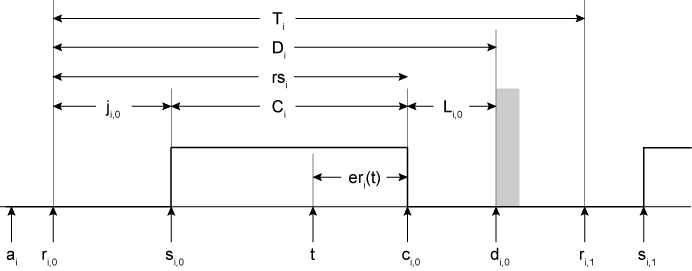
\includegraphics[width=0.7\textwidth]{master-exam-2014/figure1}
 
\item In the rate monotonic algorithm, the task with the ........... gets the highest static priority. ( Please fill in the blank )

\item In the earliest deadline algorithm, the task with the ............... gets the highest dynamic priority. ( Please fill in the blank )

\end{unteraufgaben}

\pagebreak

\aufgabe{}{10}


14.	The rate monotonic algorithm is a static priority scheduling algorithm and the earliest deadline first is a dynamic priority scheduling algorithm. Using T1 = ( 1, 4 ); T2 = ( 2, 6 ); T3 = ( 3, 8 ); where the value in parantheses are ( C, T ). Please assume the deadline to be the same as the period.

\begin{unteraufgaben}

\item	Calculate the processor utilization factor of the tasks for both the alorithms. Does the calculated factor suffice the schedulability test? Please answer why?
\item	Compute the hyperperiod of the tasks. 
\item	Fill in the chart to draw the schedulability of the tasks for both the algorithm.

\end{unteraufgaben}

\aufgabe{}{5}


Using T1 = ( 1, 4 ); T2 = ( 2, 8 ); T3 = ( 3, 12 ); where the value in parantheses are ( C, T ), please 

\begin{unteraufgaben}

\item	Calculate the processor utilization factor of the task using RM algorithm.
\item	Compute the hyperperiod of the task set. 
\item	Fill in the chart to draw the schedulability of the tasks using the RM algorithm.
\item	Can an aperiodic task with the release time of 2, deadline of 20 and computation time of 3 fit in this algorithm? Please calculate the response time of this aperiodic task.

\end{unteraufgaben}


\pagebreak

\aufgabe{}{5}

In the below precedence tasks with 9 tasks, please fill in the chart in accordance to the priority.

\begin{unteraufgaben}

\item	For a three processor system.
\item	For a four processor system. 

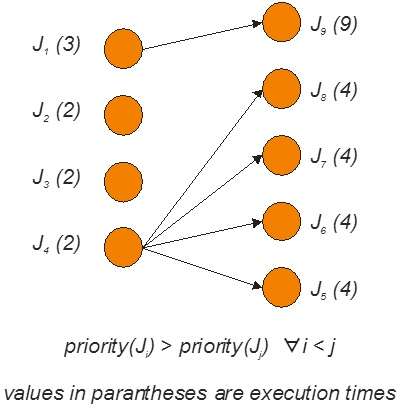
\includegraphics[width=0.5\textwidth]{master-exam-2014/figure2.jpg}

\end{unteraufgaben}


%% 3,5,6,7,8

%\pagebreak


\aufgabe{}{5}

Sketch a simple model of a real-time system and partition it into three important parts. 
Name each cluster and the interfaces between them.

\begin{tikzpicture}
\node (rect) at (0,0) [draw, text width=17 cm, minimum height=16cm]{};
\node[below right, text width=17 cm] at (rect.north west) {
    \lsg{
    Please sketch a model here
    }
   };
\end{tikzpicture}

\pagebreak

\headheight = 78pt

\aufgabe{}{2}

What is a history state? Please explain with an example.

\begin{tikzpicture}
\node (rect) at (0,0) [draw, text width=17 cm, minimum height=5cm]{};
\node[below right, text width=17cm] at (rect.north west) {
    \lsg{
    In a history state a snapshot of the contents of the data registers and the program counter is taken. \\
    Example: in a mathematical calculation with a calculator many steps are needed to reach the final result and hence the intermediate results
    are stored in the history. In case of fault during a processing of data entities, the messages from the history can be extracted to start again as if no fault had occured.
    }
   };
\end{tikzpicture}

\aufgabe{}{1}

What does signal conditioning mean? Give an example.

\begin{tikzpicture}
\node (rect) at (0,0) [draw, text width=17 cm, minimum height=4.7cm]{};
\node[below right, text width=17 cm] at (rect.north west) {
    \lsg{
    Signal conditioníng is to process meaningful data from raw data by methods such as filtering the noise, amplification of weak signals.Signal conditioning means manipulating an analog signal in such a way that it meets the requirements of the \textbf{next stage} for further processing.\\
		The plausibility check and the calibration and not part of the signal conditioning as it comes under signal processing that is one step after signal conditioning. 
    }
   };
\end{tikzpicture}

\aufgabe{}{1}

Explain the difference between polling and sampling.

\begin{tikzpicture}
\node (rect) at (0,0) [draw, text width=17 cm, minimum height=4.7cm]{};
\node[below right, text width=17 cm] at (rect.north west) {
    \lsg{ 
    In sampling, the state of the RT entity is periodically interrogated at points in time by the microcomputer. \\
    In polling, the state of the RT entity is periodically interrogated at points in time by the application. \\
    In sampling, after a successful reading of the RT entity, a trigger is generated to inform the higher layer. \\
    In polling, the value of the RT entity is acquired in a periodically running task.
    }
   };
\end{tikzpicture}

\pagebreak


\aufgabe{}{1}


Consider a combustion engine with an injection valve. The start point of fuel injection must 
be precise within 0.1 $\deg$ of the measured angular crankshaft position.
Calculate the temporal accuracy of the system if the crankshaft revolves with 6000 rpm.


\begin{tikzpicture}
\node (rect) at (0,0) [draw, text width=17 cm, minimum height=5cm]{};
\node[below right, text width=17 cm] at (rect.north west) {
    \lsg{
    2.7 $\mu$s
    }
   };
\end{tikzpicture}

\aufgabe{}{5}

Define offset, drift, drift rate, precision, and accuracy.


\begin{tikzpicture}
\node (rect) at (0,0) [draw, text width=17 cm, minimum height=10cm]{};
\node[below right, text width=17 cm] at (rect.north west) {
    \lsg{
    \textbf{Offset} : \\
		--------------\\
		Offset at microtick i between two clocks j and k with the same granularity is defined as
		the timedifference between the number of ticks of the clock j and k at microtick i. \\
		It is to be noted here that the offset is between two clocks, one of which need not be a reference clock.\\
		--------------\\
		\textbf{Drift} :  The drift of a physical clock k is determined by measuring the duration of a granule of clock k with the
		reference clock z, and dividing it by the nominal number of reference clock microticks in a granule. \\
		It is to be noted here that the drift is with reference to the reference clock.\\
		--------------\\
		\textbf{Drift rate} : The drift rate tells us how much drift is expected after a particular time. \\
		--------------\\
		\textbf{Precision} : Given an ensemble of clocks {1, 2, …, n}, the maximum offset between any two clocks of the ensemble is called
		the precision of the ensemble at microtick i \\
		--------------\\
		\textbf{Accuracy}: The offset of clock k with respect to reference clock z at microtick i is called the $accuracy_{i}$.
		}
   };
\end{tikzpicture}


\pagebreak

\aufgabe{}{5}


Global time ticks of each node are periodically resynchronized after each resynchronization interval $R_{int}$.

\begin{unteraufgaben}

\item Diagrammatically show the relation between resyncronization interval, precision and drift offset.

\item How much is the clock allowed to drift per second if a latency jitter $\varepsilon$ = 10 ps, 
a resyncronization interval $R_{int}$ = 1 sec and a precision $\pi$ = 10 ns is specified?

\item Considering that 5 clocks are in the system, what is the best precision that can be 
achieved according to the impossibility result?

\end{unteraufgaben}

\begin{tikzpicture}
\node (rect) at (0,0) [draw, text width=17 cm, minimum height=14cm]{};
\node[below right, text width=17 cm] at (rect.north west) {
    \lsg{
    .1\\
		--------------\\
    Diagram\\
    .2\\ 
		--------------\\
    $\pi$ = $\varepsilon$ + 2*$\rho$*$R_{int}$ = 4.995 * 10$^{-9}$ ns/s;\\
    .3\\
		--------------\\
    $\varepsilon$ * ( 1 - $\frac{1}{N}$ ) = 8 ps\\
    }
   };
\end{tikzpicture}


\pagebreak


\aufgabe{}{5}

\begin{unteraufgaben}

\item What is the convergence function $\phi$ in case of the central master algorithm?

\item How does the convergence function $\phi$ change in case there are k malicious clocks 
in a total of N clocks.

\item Calculate the precision $\pi$ based on the fault tolerant sync algorithm for a clock 
constellation with 1 Byzantine clock in a clock ensemble of 5 clocks. 

\end{unteraufgaben}

\begin{tikzpicture}
\node (rect) at (0,0) [draw, text width=17 cm, minimum height=15cm]{};
\node[below right, text width=17 cm] at (rect.north west) {
    \lsg{
    .1 \\
		--------------\\
    $\phi$ = $\varepsilon$ \\
    .2\\
		--------------\\
    $\phi$ = $\frac{k\pi}{(N - 2k)}$ + $\varepsilon$\\
		.3\\
		--------------\\
    $\pi$ = $\frac{(N - 2k )}{( N - 3k )}$*($\tau$ + $\varepsilon$) \\
    $\pi$ = $\frac{(3)}{(2)}$*($\tau$ + $\varepsilon$) \\
    }
   };
\end{tikzpicture}

\pagebreak

\aufgabe{}{5}

A system designer has been assigned a task to calculate the MTTF of human beings. To achieve this, 
50*10$^{4}$ human beings aged 25 years were monitored over one year. It was found that 625 of them failed ( died ) in that year.


\begin{unteraufgaben}

\item Please calculate the  failure rate $\lambda$.

\item Calculate the MTTF.

\item Please analyse your results and explain if this is realistic? If not, what would have 
been a more realistic method to calculate the MTTF?

\end{unteraufgaben}


\begin{tikzpicture}
\node (rect) at (0,0) [draw, text width=17 cm, minimum height=15cm]{};
\node[below right, text width=17 cm] at (rect.north west) {
    \lsg{
    .1\\
		--------------\\
    Subject are human beings. Since we want to calculate the life time of human beings, we would leave the
    time factor in years.
    Total number of failures = 625 \\
    Total number of years under test = 50*10$^{4}$ * 1 \\
    $\lambda$ = Total number of failures / Total number or years under test = 0.00125 failures / year \\
    .2\\ 
		--------------\\
    MTTF = $\lambda$ = 800 years. This means that the mean time to failure is 800 years. \\
    .3\\ 
		--------------\\
		The approach used by the system designer is not realistic, because the task is to calculate the MTTF of human beings and not the MTTF of human 
    beings those are 25 years old. Due to wear and tear of the body, the MTTF of other ages would reduce and hence the MTTF of the entire human cycle would
    reach a realistic number.
    }
   };
\end{tikzpicture}

\pagebreak

\aufgabe{}{5}

\begin{unteraufgaben}

\item What are the two main characteristicts of a communication channel? Please explain them.

%\item Given a bandwidth of 10 MBits/sec, a channel length of 200 m and a required protocol efficiency of 90\%, what is the maximum message length in bit that can be implemented by the media access level of a bus system

\item Consider a point-to-point link 2 km in length. At what bandwidth would the propagation delay equal 
transmit time for 100-byte packets? What about 512-byte packets?
Assume the speed of the transmission in the medium =  2*$10^{8}$ m/s,

\end{unteraufgaben}

\begin{tikzpicture}
\node (rect) at (0,0) [draw, text width=17 cm, minimum height=15cm]{};
\node[below right, text width=17 cm] at (rect.north west) {
    \lsg{
    .1\\
		--------------\\
Main characteristics of a communication channel are\\
	\textbf{Bandwidth}\\
Bandwidth indicates the number of bits that can be transmitted over a communication channel per unit time (typically described in bit/s). The bandwidth is limited by physical characteristics of the channel. For example, an unshielded twisted pair channel in a car may transmit up to 1 Mbit/s, limited by EMI constraints. A single wire channel in the same environment may only be able to transmit 10 kbit/s. An optical channel is not constrained by EMI, and can transmit many GBit/s.\\
	\textbf{Propagation delay}\\
Propagation delay is the time interval it takes for a bit to travel from one end of the channel to the other.
It is determined by the physical length of the channel and the transmission speed (electromagnetic, optical) within the channel. In vacuum, an electromagnetic wave travels at about 300.000 km/s, or 30 cm/ns. In typical cables, the transmission speed is lower than that in vacuum, about 2/3 of that value. To travel across a length of 1 km, it takes a signal about 5 $\mu$s; or it travels 20 cm/ns.\\
    .2\\
		--------------\\
    Propagation delay = Bit packet / Bandwidth = Length / Speed of communication \\
    Bandwidth = Bit packet * Speed of Communication / Length \\ 
		.\\
    Bandwidth with 100 byte packet = $\frac{100 * 8 * 2 * 10^{8}}{2000}$ = 80 Mbps \\
    Bandwidth with 512 byte packet = $\frac{512 * 8 * 2 * 10^{8}}{2000}$= 409.6 Mbps
    }
   };
\end{tikzpicture}

\pagebreak

\aufgabe{}{10}

One important parameter for many real-time computer programs is the WCET. Please explain why is it 
difficult to determine the WCET of processes in a hard-real time system. State three methods that 
have been advised to determine WCET, and discuss their limitations.

\begin{tikzpicture}
\node (rect) at (0,0) [draw, text width=17 cm, minimum height=15cm]{};
\node[below right, text width=17 cm] at (rect.north west) {
    \lsg{
    Please sketch a model here
    }
   };
\end{tikzpicture}

\pagebreak

\aufgabe{}{5}

Assuming that the start up sequence of the infotainment unit in a car depends on a CAN message sent by the central unit.
Please answer the following questions using timing formulas:

\begin{unteraufgaben}

\item  Given the maximum and minimum communication delay in a system with a local time base, how long after receiving the 
message from the central unit should the infotainment unit wait until the received message can be declared permament?

\item Assuming the above system with a global time base of granularity much smaller than the local time base, how is the  
startup time affected? Please explain your answer.

\end{unteraufgaben}

\begin{tikzpicture}
\node (rect) at (0,0) [draw, text width=17 cm, minimum height=15cm]{};
\node[below right, text width=17 cm] at (rect.north west) {
    \lsg{
    .1\\
		--------------\\
    As the time calculated should be "after" the message has been received at the infotainment unit, we have to 
    ignore the propagation delay of the message. Thus the message can be declared permanent at the infotainment unit
    when $d_{max}$ + $d_{max}$ - $d_{min}$ + $g_{l}$ time has passed.\\
    .2\\
		--------------\\
   	Since 2g << $g_{l}$, and again ignoring the propagation delay as we are concerned about the time to wait after the
   	message has been received at the infotainment unit, then time to wait for message to become permanent is \\ 
   	$t_{send}$ + $d_{max}$ + 2g \\
   	Comparing the above two formulas, we find that the time to wait reduces significantly by using a global time base.
    }
   };
\end{tikzpicture}

\pagebreak


\aufgabe{}{5}

Explain the difference between state correction and rate correction for a clock. What are the 
advantages and disadvantages for each method?

\begin{tikzpicture}
\node (rect) at (0,0) [draw, text width=17 cm, minimum height=15cm]{};
\node[below right, text width=17 cm] at (rect.north west) {
    \lsg{
Calculated correction value can be applied to local time immediately (state correction), or rate of clock can be modified such that the clock speeds up or slows down to bring it into better agreement with rest of ensemble (rate correction).\\
State correction leads to a discontinuity in the time base. If time is set back, the same time is reached again. This can cause nasty errors. Rate correction is therefore preferable.
    }
   };
\end{tikzpicture}

\pagebreak

\aufgabe{}{5}

What is the membership service in the TTP/C protocol? Explain its purpose and briefly explain how it works.

\begin{tikzpicture}
\node (rect) at (0,0) [draw, text width=17 cm, minimum height=15cm]{};
\node[below right, text width=17 cm] at (rect.north west) {
    \lsg{
\textbf{The Membership Service}\\
The membership field of a node contains one bit for each cluster node. If one out of the redundant messages is received by a receiving node, the receiving node considers the sender node operational at this membership point.\\
The node is considered operational until its next membership point in the following TDMA cycle. If a node fails within this interval, the failure is only recognized at the next membership point. Thus, the delay of the membership information is at most one TDMA cycle.
If none of the expected messages arrives with a correct CRC, then a receiver considers the sending node as failed and clears the membership bit of the sender at the end of the current SRU slot.\\
If a particular node did not receive any correct message from a sending node, e.g., because the incoming link of the receiver has failed, it assumes that this sending node has crashed, and it eliminates it from its membership vector at the end of the current SRU slot.\\
If, however, all other nodes received at least of one these messages they come to a different conclusion about the membership. This creates two cliques that cannot communicate with each other because they contain a different C-state (the membership vector is part of the C-state). \\
TTP contains a mechanism which let the majority view in such a conflict situation, i.e., the node with the failed input port, which is in the majority, is removed from the membership. Before sending a message, a node counts its negative CRC results during the last TDMA round. If more than half of the messages received have been discarded because of a failed CRC, the node assumes that its C-state differs from the majority, terminates its operation and thus leaves membership.\\
This mechanism avoids clique formation among the nodes of the ensemble. Agreement on membership is thus bound to indirect acknowledgement of message reception by the majority.\\
    }
   };
\end{tikzpicture}

\pagebreak

\lsg{
Full page solution
}

%% 3,5,6,7,8

%\pagebreak

\aufgabe{Attempt any 10 questions}{20}

You are asked to design a real time distributed network with 3 nodes. All the nodes are equipped with a low speed CAN controller ( TJA1054T ) and a host CPU as shown in the figure. Pin Number 16 and Pin number 17 are the Can Rx and Can Tx pins on the host CPU respectively.
%\begin{figure}[ht]
%\begin{center}
$\begin{array}{cc}
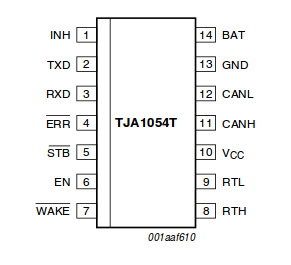
\includegraphics[width=6cm]{files-2016/tja1054t} &
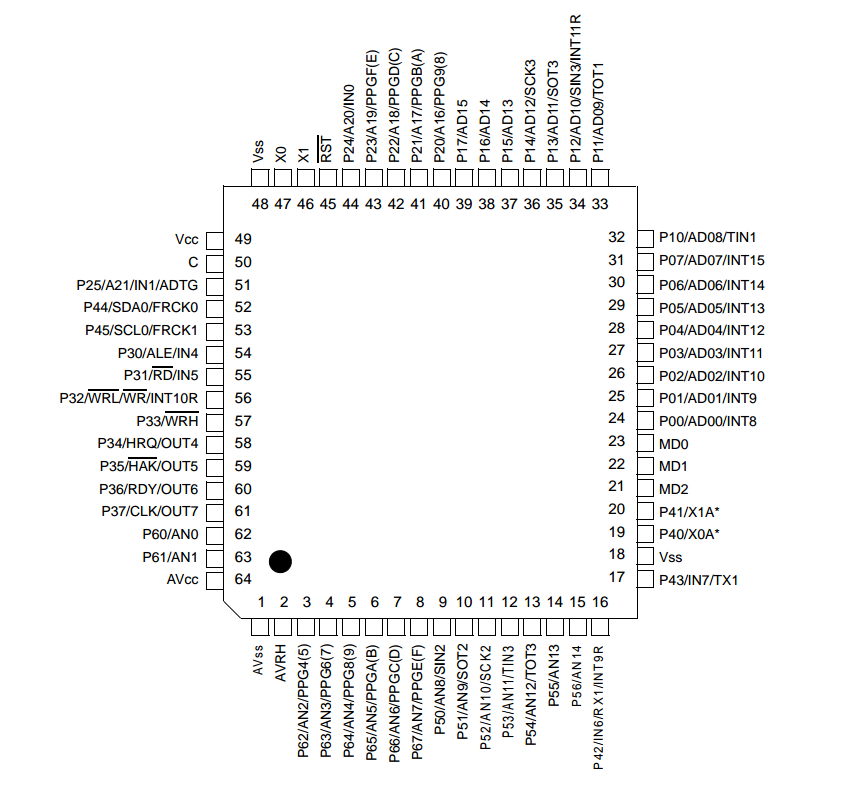
\includegraphics[width=8cm]{files-2016/fujitsu}
\end{array}$
%\end{center}
%\end{figure}

\begin{tikzpicture}
\draw[thick,<->] (0,10) -- (15,10) node[anchor=north west] {CAN L};
\draw[thick,<->] (0,11) -- (15,11) node[anchor=north west] {CAN H};;
\end{tikzpicture}

\begin{enumerate}
    \item Draw how a real time node looks like and list the main components in such a node.
    \item In the fig above, connect the CAN receive and transmit pins on the host CPU with those on the communication controller.
    \item In the fig above, connect the communication bus with the appropriate pins on the communication controller.
    \item Now, in the page below, make a new distributed network diagram with 3 nodes by connecting all of them with each other via the communication bus.
    \item Assign a CAN ID to each node and discuss how the nodes access the bus in case of collisions?
\end{enumerate}

\pagebreak

\headheight = 78pt

\begin{tikzpicture}
\node (rect) at (0,0) [draw, text width=16.6 cm, minimum height=24cm]{};
\node[below right, text width=16.6 cm] at (rect.north west) {
    \lsg{
\begin{tikzpicture}[squarednode/.style={rectangle, draw=red!60, fill=red!5, very thick, minimum size=5mm}]
%Nodes
\node[squarednode]      (hostcpu)                              {2};
\node[squarednode]      (coummunication)                              {4};
%\node[roundnode]        (uppercircle)       [above=of maintopic] {1};
%Lines
\draw[->] (coummunication.south) -- (hostcpu.north);
%\draw[->] (maintopic.east) -- (rightsquare.west);
%\draw[->] (rightsquare.south) .. controls +(down:7mm) and +(right:7mm) .. (lowercircle.east);
\end{tikzpicture}
    }
   };
\end{tikzpicture}


Each node is connected in parallel to a 12V DC battery with a capacity of 5400 mAh. Each node has an energy consumption of 100 mAh in operational mode and 1 mAh in standby mode.

\begin{enumerate}
    \addtocounter{enumi}{5}
%    \setcounter{enumii}{4}
    \item Extend your block diagram above by connecting the battery unit to the nodes.
    \item Assuming that the car has no charger unit, how much energy does the battery still have after 20 hours, if the car is in the operational mode for 15 hours and in standby mode for 5 hours ?
\end{enumerate}

\begin{tikzpicture}
\node (rect) at (0,0) [draw, text width=16.6 cm, minimum height=5cm]{};
\node[below right, text width=16.6 cm] at (rect.north west) {
    \lsg{
    Please sketch a model here
    }
   };
\end{tikzpicture}


Assuming Node 3, starts sending Error Frames on the bus. 
\begin{enumerate}
    \addtocounter{enumi}{7}
    \item How does the CAN driver know about the error frames on the bus and what measures would you take to make sure that all the nodes can still communicate with each other? Hint > Please see the chip diagram.
    \item Discuss why a terminating resistance is important in a multi-node communication network system.
\end{enumerate}

\begin{tikzpicture}
\node (rect) at (0,0) [draw, text width=16.6 cm, minimum height=6cm]{};
\node[below right, text width=16.6 cm] at (rect.north west) {
    \lsg{
    Please sketch a model here
    }
   };
\end{tikzpicture}
 

The two farthest nodes are 5 m away from each other. The low speed CAN transciever can transmit and receive messages with a bandwidth of 125 KBit / second. The speed of the transmission of the bits is 2/3 of the speed of the light and the message length is 100 bits.

\begin{enumerate}
    \addtocounter{enumi}{9}
    \item What is the bit length of the two farthest nodes? 
    \item Calculate the best channel utilization in percentage.
\end{enumerate}

\begin{tikzpicture}
\node (rect) at (0,0) [draw, text width=16.6 cm, minimum height=6cm]{};
\node[below right, text width=16.6 cm] at (rect.north west) {
    \lsg{
    Please sketch a model here
    }
   };
\end{tikzpicture}


TDMA is Time Division Multiple Access and CSMA/CA is Carrier Sense Multiple Access / Collision Avoidance. 

\begin{enumerate}
    \addtocounter{enumi}{11}
    \item Name 5 important parameters which you would need to know, before choosing the right protocol such as the one above
\end{enumerate}

\begin{tikzpicture}
\node (rect) at (0,0) [draw, text width=16.6 cm, minimum height=6cm]{};
\node[below right, text width=16.6 cm] at (rect.north west) {
    \lsg{
    Please sketch a model here
    }
   };
\end{tikzpicture}

\pagebreak

\aufgabe{}{10}


You are given a quartz which oscillates at the rate of 32768 ticks per second. 

Your job is to make 3 local clocks each with a macro-granularity of 512 ticks. Each clock drifts differently at a drift rate $\rho$ $10^{-9}$ s/s, $2*10^{-9}$ s/s, $3*10^{-9}$ s/s respectively.

\begin{enumerate}
    \addtocounter{enumi}{0}
\item What is the granularity of the reference clock?
\item What is the granularity of the local clock?
\item What is the minimum time and the maximum time that can be measured in one of the local clock with a 32 bit variable?
\item What is the precision of the clock ensemble over an interval of interest of 1 second?
\end{enumerate}

\begin{tikzpicture}
\node (rect) at (0,0) [draw, text width=16.6 cm, minimum height=13cm]{};
\node[below right, text width=16.6 cm] at (rect.north west) {
    \lsg{
    Please sketch a model here
    }
   };
\end{tikzpicture}

The clocks are synchronized to the reference clock via a communication bus. The latency jitter between the the reference clock and the local clock is $10^{-12}$ s.
The formula for drift offset is $\Gamma =  2 * \rho * R_{int}$

\begin{enumerate}
    \addtocounter{enumi}{4}
\item Calculate the synchronization interval according the central master algorithm of one of the local clock of your choice.

\end{enumerate}

\begin{tikzpicture}
\node (rect) at (0,0) [draw, text width=16.6 cm, minimum height=6 cm]{};
\node[below right, text width=16.6 cm] at (rect.north west) {
    \lsg{
    Please sketch a model here
    }
   };
\end{tikzpicture}

\aufgabe{}{10}

Consider a combustion engine with an injection valve. The start point of fuel injection must be precise within $2\degree$ of the measured angular crankshaft position.
\begin{enumerate}
\item Calculate the temporal accuracy of the system, if the crankshaft revolves with 6000 rpm.
\end{enumerate}

\begin{tikzpicture}
\node (rect) at (0,0) [draw, text width=16.6 cm, minimum height=7cm]{};
\node[below right, text width=16.6 cm] at (rect.north west) {
    \lsg{
    Please sketch a model here
    }
   };
\end{tikzpicture}

Considering an update rate $d_{update}$ of 10 $\mu$s, WCET of the sender as 500 ns and the WCET of the receiver as 1500 ns and the worst case latency of the communication bus as 18 $\mu$s, discuss the type of the image derived ( phase sensitive or phase insensitive ).

\begin{enumerate}
\addtocounter{enumi}{1}
\item Discuss the type of the image if the high level PAR protocol of the RT transaction between the sender and the receiver allows a maximum of 2 retry.
\item How can you solve the problem of phase insensitive images?
\end{enumerate}


\begin{tikzpicture}
\node (rect) at (0,0) [draw, text width=16.6 cm, minimum height=15cm]{};
\node[below right, text width=16.6 cm] at (rect.north west) {
    \lsg{
    Please sketch a model here
    }
   };
\end{tikzpicture}

\pagebreak

\aufgabe{}{20}

Consider a task set T composed of the following three periodic tasks:
\begin{itemize}
\item T1(0, 1, 6) (release time, computation time, deadline)
\item T2(0, 2, 10)
\item T3(0, 5, 15)
\end{itemize}

\begin{enumerate}
\item Compute the major cycle of the task set. 
\item Verify the schedulability under the EDF algorithm. 
\item Build the schedule.
\end{enumerate}

Consider the following aperiodic tasks:
\begin{itemize}
    \item T4(1, 2, 29) (release time, computation time, deadline)
    \item T5(13, 2, 10)
    \item T6(21, 4, 9)
\end{itemize}

\begin{enumerate}
\addtocounter{enumi}{3}
\item \textbf{\underline{All}} aperiodic tasks are scheduled in the background together with the main tasks. Compute the response times of tasks T4, T5, and T6. 
\item Do you think that any of the aperiodic task would not be able to meet the deadline?
\end{enumerate}




\aufgabe{}{10}

According to the NASA Managers, the Space shuttle Challenger had a failure rate of 1 in 100000 hours. However, Richard Feynman who was investigating the explosion of the space shuttle that led to the killing of all crew members, reported a failure rate of 1 in 200 hours.

\begin{enumerate}
\item Calculate the MTTF as per the NASA managers?
\item Calculate the MTTF as per Richard Feynman?
\item Calculate the reliability of the space shuttle 1 hour after the shuttle is switched on as per the NASA managers?
\item Calculate the reliability of the space shuttle 1 hour after the shuttle is switched on as per Richard Feynman?
\item Why is it important to carefully calculate the MTTF for highly critical systems?
\end{enumerate}

\begin{tikzpicture}
\calcremainingheight
\node (rect) at (0,0) [draw, text width=16.6 cm, minimum height=\remainingheight]{};
\node[below right, text width=16.6 cm] at (rect.north west) {
    \lsg{
%    MTTF = $1/\lambda$ \\
%    \lambda_{Nasa Managers} = $1/100000$ hours. Hence MTTF = 100000 hours\\
%    \lambda_{Feynman} = $1/200$ hours. Hence MTTF = 200 hours. \\\\
%    The MTTF of the system calculate according to Feynman is quite small and hence such a system should not have been launched. For a safety critical system, the MTTF should be ideally in 100 thousands of hours. \\
%    Reliablility R(t) = $\exp^{-\lambda(t-t\_{0}}$ \\
%    Reliablity_{Nasa Managers}(1) = $\exp^{-(1/100000)*(1-0}$ \\
%    Reliablity_{Feynman}(1) = $\exp^{-(1/200)*(1-0}$ \\
    }
   };
\end{tikzpicture}

\pagebreak

\aufgabe{}{20}

The US division of Mercedes \& Bosch teamed up to create Robo-Taxis ( driverless taxis ) in April this year. There are innumerous challenges in driverless cars.
One such challenge is driving in the city with lots of pedesterians around. Your job is to focus on the system design, where you can detect the movement of the pedesterians,
and correspondingly steer / brake or accelerate the car. 

\begin{enumerate}

\item Depict the design of your system with the help of 3 components of the real-time systems.
\item Define hard and soft deadlines through examples. Discuss if your designed system should have hard deadlines? If so, why?
\item List some of your system's functional and non-functional requirement. Please elaborate the temporal requirement falling under the category of non-functional requirements.
\item What kind of sensors would you employ to detect the pedesterians? 
\item How can you monitor the failure of components such as sensors after the car has rolled out of production?

\end{enumerate}

\begin{tikzpicture}
\calcremainingheight
\node (rect) at (0,0) [draw, text width=16.6 cm, minimum height=\remainingheight]{};
\node[below right, text width=16.6 cm] at (rect.north west) {
    \lsg{
    Please sketch a model here
    }
   };
\end{tikzpicture}

\newpage

Contd...

\begin{tikzpicture}
\calcremainingheight
\node (rect) at (0,0) [draw, text width=16.6 cm, minimum height=\remainingheight]{};
\node[below right, text width=16.6 cm] at (rect.north west) {
    \lsg{
    Please sketch a model here
    }
   };
\end{tikzpicture}

\pagebreak

Nodes with identical sensors are replicated to improve the reliability of the whole system, so that even if one of the sensor fails, the system will still continue working based on the other sensors. 

\begin{enumerate}
\item Draw a block diagram to show how these different nodes are communicating via a communication bus.
\item Explain the difference between state messages and event messages. Mention some state messages with respect to your system.
\end{enumerate}


\begin{tikzpicture}
\calcremainingheight
\node (rect) at (0,0) [draw, text width=16.6 cm, minimum height=\remainingheight]{};
\node[below right, text width=16.6 cm] at (rect.north west) {
    \lsg{
    Please sketch a model here
    }
   };
\end{tikzpicture}

\pagebreak

Following are 4 dependant tasks and 1 independent task to realise your software.
The semantic for the task set is ( Release time, Computation Time, Time Period )
\begin{description}
\item[$\bullet$ Task A] : Sensor acquisition task ( 0, 50, 100 ) 
\item[$\bullet$ Task B] : Sensor processing task ( 0, 20, 100 ) 
\item[$\bullet$ Task C] : Communication Task ( 0, 20, 100 )
\item[$\bullet$ Task D]: Decision Task ( 0, 10, 100 )
\end{description}
A -> B -> C -> D ( 
Dependancy graph )
\begin{description}
\item[$\bullet$ Task E] : Independent Task: Diagnostic Task ( 0, 50, 3000 )
\end{description}

\begin{enumerate}
\item Compute the Hyperperiod of all the task set.
\item Calculate the processor utilisation factor ( Ratio of computation and time period of all tasks ) for the combined task sets.
\item Discuss if its possible to run the above task set in a single core system? If not, then how many cores do you need? 
\end{enumerate}


\begin{tikzpicture}
\calcremainingheight
\node (rect) at (0,0) [draw, text width=16.6 cm, minimum height=\remainingheight]{};
\node[below right, text width=16.6 cm] at (rect.north west) {
    \lsg{
    Please sketch a model here
    }
   };
\end{tikzpicture}

\pagebreak

\aufgabe{}{10}

In 2017, ten atomic clocks ( all manufactured from SpetraTime ) failed to oscillate in the European Union’s Galileo navigation satellites.
The possible cause is thought to be waking up the satellites after deep sleep which leads to a short circuit in the clock circuitry.
 
\begin{enumerate}
\item What is meant by oscillations in a clock?
\item What role does a clock play in the powermanagement of a CPU?
\item Assuming a clock drift at the rate of $10^{-5}$ sec/sec, what would be the offset of the clock after 1 hour?
\item In an ensemble of 4 clocks with a latency jitter of $5*10^{-5}$ seconds, the system designer wants to maintain a precision of 36 ms. In what intervals should the clock be synchronised?
\item Assuming 4 identical clocks are employed from the same manufacturer in your design, and one of the clock is Byzantine. Calculate the synchronisation interval to maintain the required precision.
%$R_{int}$ = 
\end{enumerate}

\begin{tcolorbox}[height fill, title=Your solution]
    \lsg{
    Please sketch a model here
    }
\end{tcolorbox}

%\begin{tikzpicture}
%\calcremainingheight
%\node (rect) at (0,0) [draw, text width=16.6 cm, minimum height=\remainingheight]{};
%\node[below right, text width=16.6 cm] at (rect.north west) {
%    \lsg{
%    Please sketch a model here
%    }
%   };
%\end{tikzpicture}

\pagebreak

\aufgabe{}{10}
\begin{enumerate}

\item Draw the different layers of OSI Reference Model.
\item In a bus communication, discuss 2 methods, how the bus access is resolved at the time when two nodes want to send their data at the same time?
\item For a message length of 100 bytes, bandwidth of 1 Mbit/second and the distance between two nodes as 10 meters, calculate the bus efficiency. Assume speed of light in the medium as 2/3rd of speed of light.
\item How does the bus efficiency change, if the bandwidth is 1 Gbit/second?
\item How can you improve the bandwidth of the transmission from 1 Mbit/second to for example 10 Mbit/second through software methods? 
\end{enumerate}

\begin{tikzpicture}
\calcremainingheight
\node (rect) at (0,0) [draw, text width=16.6 cm, minimum height=\remainingheight]{};
\node[below right, text width=16.6 cm] at (rect.north west) {
    \lsg{
    Please sketch a model here
    }
   };
\end{tikzpicture}

\pagebreak

\begin{tikzpicture}
\calcremainingheight
\node (rect) at (0,0) [draw, text width=16.6 cm, minimum height=\remainingheight]{};
\node[below right, text width=16.6 cm] at (rect.north west) {
    \lsg{
    Please sketch a model here
    }
   };
\end{tikzpicture}


\aufgabe{}{10}
\begin{enumerate}

\item What is a context switch?
\item What is the process of context switch between a running task and an interrupt?
\item Is the process of context switch between a running task and an interrupt the same as a context switch between two tasks?
\item What triggers a task switch in a round robin scheduling algorithm?
\item What is one major advantage of a multi core system over a single core system with respect to context switches?
\end{enumerate}

\begin{tikzpicture}
\calcremainingheight
\node (rect) at (0,0) [draw, text width=16.6 cm, minimum height=\remainingheight]{};
\node[below right, text width=16.6 cm] at (rect.north west) {
    \lsg{
    Please sketch a model here
    }
   };
\end{tikzpicture}

\newpage


\begin{tcolorbox}[height fill, title=Your solution]
    \lsg{
    Please sketch a model here
    }
\end{tcolorbox}

\newpage


\begin{tikzpicture}
\calcremainingheight
\node (rect) at (0,0) [draw, text width=16.6 cm, minimum height=\remainingheight]{};
\node[below right, text width=16.6 cm] at (rect.north west) {
    \lsg{
    Please sketch a model here
    }
   };
\end{tikzpicture}


\end{document}
